%%%%%%%%%%%%%%%%%%%%%%%%%%%%%%%%%%%%%%%%
% Beamer Presentation
% LaTeX Template
% Version 1.0 (10/11/12)
%
% This template has been downloaded from:
% http://www.LaTeXTemplates.com
%
% License:
% CC BY-NC-SA 3.0 (http://creativecommons.org/licenses/by-nc-sa/3.0/)
%
%%%%%%%%%%%%%%%%%%%%%%%%%%%%%%%%%%%%%%%%%

%----------------------------------------------------------------------------------------
%	PACKAGES AND THEMES
%----------------------------------------------------------------------------------------
\documentclass[10pt]{beamer}
%\PassOptionsToPackage{height=0.5cm}{beamerouterthemesidebar}
\DeclareOptionBeamer{compress}{\beamer@compresstrue}
\ProcessOptionsBeamer
\mode<presentation> {

% The Beamer class comes with a number of default slide themes
% which change the colors and layouts of slides. Below this is a list
% of all the themes, uncomment each in turn to see what they look like.

%\usetheme{default}
%\usetheme{AnnArbor}
%\usetheme{Antibes}
%\usetheme{Bergen}
%\usetheme{Berkeley}
%\usetheme{Berlin}
%\usetheme{Boadilla} %nice
%\usetheme{CambridgeUS}
%\usetheme{Copenhagen}
%\usetheme{Darmstadt}
%\usetheme{Dresden} %nice
%\usetheme{Frankfurt} %nice
%\usetheme{Goettingen}
%\usetheme{Hannover}
%\usetheme{Ilmenau}
%\usetheme{JuanLesPins} %nice
%\usetheme{Luebeck}
\usetheme{Madrid} %or this one
%\usetheme{Malmoe}
%\usetheme{Marburg}
%\usetheme{Montpellier}
%\usetheme{PaloAlto}
%\usetheme{Pittsburgh}
%\usetheme{Rochester}
%\usetheme{Singapore}
%\usetheme{Szeged}
%\usetheme{Warsaw}

% As well as themes, the Beamer class has a number of color themes
% for any slide theme. Uncomment each of these in turn to see how it
% changes the colors of your current slide theme.

%\usecolortheme{albatross}
%\usecolortheme{beaver}
%\usecolortheme{beetle}
%\usecolortheme{crane}
%\usecolortheme{dolphin}
%\usecolortheme{dove}
%\usecolortheme{fly}
%\usecolortheme{lily}
%\usecolortheme{orchid}
%\usecolortheme{rose}
%\usecolortheme{seagull}
%\usecolortheme{seahorse}
%\usecolortheme{whale}
%\usecolortheme{wolverine}
%\usecolortheme{spruce}
%\useoutertheme{smoothtree} % smoothtree
\useinnertheme{rounded}
\definecolor{TIblue}{HTML}{153291} % UBC Blue (primary)
\definecolor{UBCblue}{HTML}{8A9ACD}
\usecolortheme[named=TIblue]{structure}
\setbeamercolor{section in toc}{fg=TIblue} % TOC sections
\setbeamercolor{subsection in head/foot}{bg=TIblue,fg=TIblue}
\setbeamercolor{palette primary}{bg=TIblue,fg=white}
\setbeamercolor{palette secondary}{bg=TIblue,fg=white}
\setbeamercolor{palette tertiary}{bg=TIblue,fg=white}
\setbeamercolor{palette quaternary}{bg=UBCblue,fg=white}
\setbeamercolor{block title}{bg=UBCblue,fg=black}
%\setbeamertemplate{footline} % To remove the footer line in all slides uncomment this line
\setbeamertemplate{footline}[frame number] % To replace the footer line in all slides with a simple slide count uncomment this line
\setbeamertemplate{navigation symbols}{} % To remove the navigation symbols from the bottom of all slides uncomment this line
}
\newcommand{\red}[1]{\textcolor{red}{#1}} 
\newcommand{\blue}[1]{\textcolor{blue}{#1}}
\usepackage{graphicx} % Allows including images
\usepackage{booktabs} % Allows the use of \toprule, \midrule and \bottomrule in tables
\usepackage{natbib}
\usepackage[utf8]{inputenc}
\usepackage{hyperref}
\usepackage{bbm}
\usepackage{bm}
\usepackage{amsmath}
\usepackage{caption}
\usepackage{siunitx,booktabs,threeparttable}
\usepackage{appendixnumberbeamer}
\captionsetup[table]{justification=raggedright,singlelinecheck=off}
\sisetup{separate-uncertainty=true}
\DeclareMathOperator*{\argmax}{arg\max}
\setbeamertemplate{caption}[numbered]

%----------------------------------------------------------------------------------------
%	TITLE PAGE
%----------------------------------------------------------------------------------------

\title[Sample Selection Bias in Dyadic Regressions] {Correcting for Sample Selection Bias in Dyadic Regressions} % The short title appears at the bottom of every slide, the full title is only on the title page
\subtitle[]{An Application to Gravity Models}
\author{Gabriela Mara Miyazato Szini \\ \small{\textit{g.m.m.szini@uva.nl}}} % Your name

\titlegraphic{
\includegraphics[width=0.25\textwidth]{ti_logoblok.jpg}\hspace{2em}
\includegraphics[width=0.2\textwidth]{uvalogo.jpg}}


\institute[] % Your institution as it will appear on the bottom of every slide, may be shorthand to save space
{
Supervised by: Prof. Dr. Frank Kleibergen % Your email address
}
\date{\today} % Date, can be changed to a custom date
% add here more packages or macros if needed

\begin{document}
\begin{frame}
  \titlepage % Print the title page as the first slide
\end{frame}

\section{Introduction}
\begin{frame}
    \frametitle{Motivation}
    \begin{itemize}
        \item    \cite{tinbergen1962shaping} established gravity equations: used to estimate models of international trade flows. Particularly, to infer the effects of trade barriers on flows.\\~\\  \pause
        \item \textbf{Before \cite{helpman2008estimating}:} studies only considered observations with positive trade flows when estimating the model, without imposing any special treatment on it. \\~\\ 
        \item \textbf{\cite{helpman2008estimating}:} correct for sample selection using the standard \cite{heckman1979sample} approach. \hyperlink{Gravity model}{\beamerbutton{Gravity model}}\\~\\ \pause
        \item \textbf{What is the remaining problem?} \\
        The inclusion of two-way fixed effects when correcting for sample selection through \cite{heckman1979sample} approach leads to incidental parameter problem (\cite{neyman1948consistent})\\~\\  \pause
        \item \textbf{Main aim:} propose estimators that are not contaminated by this problem.
    \end{itemize}


  \end{frame}

  \begin{frame}
      \frametitle{Aim of the study}
      \begin{itemize}
          \item<1->  Define a model to any dyadic data with sample selection. \\~\\ 
          \item<2->  Outline the incidental parameter problem that arises when employing the standard \cite{heckman1979sample} aproach. \\~\\ 
          \item<3->  First stage of sample selection correction: method based on conditional likelihood estimators of \cite{charbonneau2017multiple}. \\~\\ 
          \item<4->  Propose new approaches to the second stage of sample selection correction: 
          \begin{itemize}
              \item Hybrid estimates of fixed effects + Lee's transformation.
              \item Modification to \cite{kyriazidou1997estimation}. \\~\\ 
          \end{itemize}
          \item<5-> Simulation exercise indicates that new approaches reduces the biases in the estimates. 
      \end{itemize}
  \end{frame}
\section{A generalized model of dyadic interactions}
\begin{frame}
    \frametitle{Model of dyadic interactions}
    \begin{align*}
        y_{1,ij,t} = x_{1,ij,t}'\beta_1 + \vartheta_i + \chi_j + u_{ij,t} \quad \text{(Observation equation)}
    \end{align*}
    \begin{align*}
        y_{2,i j,t}= \mathbbm{1} (y_{2,i j,t}^{**} > 0)
    \end{align*}
    \begin{align*}
        y_{2,i j,t}^{**}=x_{2,ij,t}'{\beta_2^*}  +\xi_{i}^*+\zeta_{j}^*+\eta^*_{i j,t} \quad \text{(Selection equation)}
        \label{eq:model3}
    \end{align*}
    \begin{equation*}
    \hspace{10000pt minus 1fil} (i = 1,...N; j=1,...N, t=1,...T, i \neq j)\hfilneg
    \end{equation*}
    \begin{itemize}
        \item $y_{1,ij,t}$ is observed only when $y_{2,i j,t} = 1$. 
        \item $x_{1,ij,t}$ and $x_{2,ij,t}$ are vectors  of $k$ and $q$ explanatory variables.
        \item $\beta_1 \in \mathbbm{R}^k$ and $\beta_2^* \in \mathbbm{R}^q$
        \item $\chi_j$, $\vartheta_i$, $\xi_i^*$ and $\zeta_j^*$ are fixed effects.
    \end{itemize} \pause
    \textbf{Main features:} 
    \begin{itemize}
        \item Unobserved individual effects may depend on other variables arbitrarily. 
        \item Errors of equations might be correlated.
        \item Directed links/outcomes.
        \item Selection equation indicates a network formation model with degree heterogeneity.
    \end{itemize}
  \end{frame}
\section{\cite{heckman1979sample}'s approach and the incidental parameter problem}


\begin{frame}
    \frametitle{Currently in the literature: Heckman's two-step approach}
    \begin{block}{Assumption:} 
        $$\mathbbm{E}[u_{ij,t} {\eta_{ij,t}^*}] = 
        \begin{cases}
            \sigma_{u\eta^*} \text{ if } i=i', j=j', t=t'\\
            0 \text{ otherwise}\\
            \end{cases}$$
      \end{block}
    We can rewrite the observation equation as:
    \begin{align*} 
        &\mathbbm{E}[y_{1,ij,t} \rvert x_{1,ij,t}, \vartheta_i, \chi_j, y_{2,i j,t}= 1] \\ 
        &=  x_{1,ij,t}'\beta_1 + \vartheta_i + \chi_j + \mathbbm{E} [u_{ij,t} \rvert \eta^*_{i j,t} \geq \underbrace{-x_{2,ij,t}'{\beta_2^*}  -\xi_{i}^*-\zeta_{j}^*}_{z_{ij,t}}] \nonumber
    \end{align*}  \pause
    Further assuming that the conditional expectation in the last term is an unknown, smooth function $\varphi_{ij,t}$:
    \begin{align*}
        y_{1,ij,t} =  x_{1,ij,t}'\beta_1 + \vartheta_i + \chi_j + \varphi_{ij,t}(z_{ij,t}) + \nu_{ij,t},
    \end{align*}
    \noindent by construction, $\mathbbm{E}[\nu_{ij,t} \rvert x_{1,ij,t}, \vartheta_i, \chi_j, \varphi_{ij,t}(z_{ij,t}), y_{2,i j,t}^{**} > 0] = 0$. \pause
    \\~\\
    \textbf{Identification:} either the function $\varphi_{ij,t}$ is specified or additional variables that satisfy exclusion restriction from the observation equation are included in $x_{2,ij,t}$.   
\end{frame}

\begin{frame}
    \frametitle{Currently in the literature: Heckman's two-step approach}
    Introducing functional form for $\varphi_{ij,t}$ through additional distributional assumptions: 
    \begin{block}{Assumption:}
        The error term $u_{ij,t}$ is i.i.d. over $ij$ and $t$, such that $u_{ij,t} \sim N(0, \sigma_u^2)$. \\
        The error term $\eta_{ij,t}^*$ is i.i.d. over $ij$ and $t$, such that $\eta_{ij,t}^* \sim N(0, 1)$.
    \end{block} \pause
    From the standard results of the bivariate normal distribution:
    \begin{align*}
        y_{1,ij,t} =  x_{1,ij,t}'\beta_1 + \vartheta_i + \chi_j + \sigma_{u\eta^*} \lambda_{ij,t}(z_{ij,t}) + \nu_{ij,t}
    \end{align*}
    \noindent where: $\lambda_{ij,t}(z_{ij,t}) = \frac{\phi(z_{ij,t})}{1 - \Phi(z_{ij,t})} = \frac{\phi(z_{ij,t})}{\Phi(-z_{ij,t})}$ is the inverse Mills-ratio. 
\end{frame}

\begin{frame}
    \frametitle{Currently in the literature: Heckman's two-step approach}
    \cite{heckman1979sample}'s approach in a nutshell:
    \begin{itemize}
        \item \textbf{Stage 1:} Estimate selection equation by MLE (probit).
        \item \textbf{Stage 2:} Obtain inverse Mills-ratio and estimate observation equation by FGLS. \\~\\
    \end{itemize}  \pause
    Taking into account an \textbf{estimated value} of $\lambda_{ij,t}(z_{ij,t})$:
    \begin{align*}
        y_{1,ij,t} = x_{1,ij,t}'\beta_1 + \vartheta_i + \chi_j + \sigma_{u\eta^*} \hat{\lambda}_{ij,t} + \sigma_{u\eta^*} ({\lambda}_{ij,t} - \hat{\lambda}_{ij,t}) + \nu_{ij,t}
    \end{align*}
    We can interpretate $\sigma_{u\eta^*} ({\lambda}_{ij,t} - \hat{\lambda}_{ij,t}) + \nu_{ij,t}$ as the error term of this equation. \pause
    \begin{block}{Theorem 1:}
        The estimator of $\beta_1$ will be an asymptotically unbiased estimator, i.e., will converge to a limiting distribution centered around its true value only if $\mathbbm{E} [ ({\lambda}_{ij,t} - \hat{\lambda}_{ij,t}) ] = 0$.
    \end{block} 

    \hyperlink{Heckman}{\beamerbutton{Heckman's steps}}
\end{frame}
\begin{frame}
    \frametitle{Which is the problem? The incidental parameter problem}
    \textbf{Fixed effects estimators in nonlinear models suffer from the \textbf{incidental parameter problem} (\cite{neyman1948consistent})}. \pause
    \\~\\
    \textbf{How does this problem arise?}\\
    Denote:
    $$\Bar{\beta}^*_2 = \argmax_{\beta^*_2 \in \mathbb{R}^{\text{dim} \beta^*_2}} \mathbb{E}_\omega \Big[\mathcal{L} (\beta^*_2, \hat{\omega}_{NN}^*(\beta^*_2)) \Big]$$
    Using an asymptotic expansion for smooth likelihoods under appropriate regularity conditions (\cite{fernandez2016individual}) \hyperlink{Asymptotic}{\beamerbutton{Asymptotic expansion}}
    :
    \begin{align*} 
        \Bar{\beta}_2^* = \beta_{2,0}^* + \frac{\Bar{B}_\infty}{(N-1)T} + \frac{\Bar{D}_\infty}{(N-1)T} + \text{o}_P(((N-1)T)^{-1})
    \end{align*}
    For some constants $\Bar{B}_\infty$ and $\Bar{D}_\infty$. \pause
    By the properties of the maximum likelihood estimator:
    \begin{align*}
        \sqrt{N(N-1)T} (\hat{\beta}_2^* - \Bar{\beta}_2^*) \xrightarrow{d} N(0, \Bar{V_B}_\infty)
    \end{align*}
    For some $\Bar{V_B}_\infty$. By Slutsky Theorem:
    \begin{align*} 
        \sqrt{N(N-1)T} (\hat{\beta}_2^* - \beta_{2,0}^*) \xrightarrow{d} N\Big( \frac{\Bar{B}_\infty}{\sqrt{T}} + \frac{\Bar{D}_\infty}{\sqrt{T}}, \Bar{V_B}_\infty\Big) \nonumber
    \end{align*}
\end{frame}


\begin{frame}
    \frametitle{Which is the problem? The incidental parameter problem}
    As $N \xrightarrow{} \infty$ and considering fixed $T$:
    \\~\\
    \begin{itemize}
        \item $\hat{\beta}_2^* \xrightarrow{p} \beta_{2,0}^*$ : estimates are consistent.
        \item \textbf{But} the estimates converge to a distribution that is not centered at the true parameter value, which leads to incorrect asymptotic confidence intervals.
        \\~\\
    \end{itemize} \pause
    The source of the problem is that the estimates of the nuisance parameters converge at a slower rate than the structural parameters. \pause
    \begin{block}{Conjecture 1:}
        The asymptotic bias in the estimates of $\beta_{2}^*$ carries over both to the estimates of the fixed effects, $\hat{\omega}_{NN}^*$ and to the estimates of the inverse Mills-ratio, $\hat{\lambda}_{ij,t}$.
    \end{block}
    \textbf{Conditions of Theorem 1 do not hold.}
\end{frame}


\section{First stage: conditional logit estimation of \cite{charbonneau2017multiple}}
\begin{frame}
    \frametitle{Our proposed methods: Outline}
    \begin{enumerate}
        \item \textbf{First stage: conditional logit estimation of \cite{charbonneau2017multiple}.}
        \begin{itemize}
            \item \textbf{Differences out the fixed effects $\xrightarrow[]{}$ free of incidental parameter problem.}\\~\\ 
        \end{itemize}
        \item Second stage: given estimates of first stage, we propose two methods.
        \begin{itemize}
            \item Hybrid approach to retrieve FE of first stage + Lee's transformation to apply Heckman even when errors are logistic distributed.
            \item A modification to the \cite{kyriazidou1997estimation} approach that relies on the idea of differencing out the selection effects.
        \end{itemize}
    \end{enumerate}
\end{frame}
\begin{frame}
    \frametitle{{Conditional logit estimation of \cite{charbonneau2017multiple}}}
\textbf{Main idea:} difference out two-way fixed effects in selection equation. \\
\textbf{Result:} obtain estimates of $\beta_2^*$ that are not contaminated by the incidental parameters problem. 
\\~\\ \pause
Modify Assumption on the distribution of $\eta_{ij}^*$ to: 
\begin{block}{Assumption:}
    The idiosyncratic terms $\eta_{ij}^*$ are i.i.d. across $ij$ and follow a standard logistic distribution conditional on the regressors and fixed effects.
\end{block}
For simplicity: consider only one period $t$. \\~\\ \pause
Assumption implies that:
\begin{align*}
    \text{Pr}(y_{2,ij} = 1 \rvert x_{2}, \xi^*, \zeta^*, \beta_2^*) = \frac{\exp (x_{2,ij}'{\beta_2^*}  +\xi_{i}^*+\zeta_{j}^*)}{1 + \exp (x_{2,ij}'{\beta_2^*}  +\xi_{i}^*+\zeta_{j}^*)}
\end{align*}
\noindent where $x_{2}$ is the vector of observations $x_{2,ij}$ for all possible pairs $ij$.

\end{frame}

\begin{frame}
    \frametitle{{Conditional logit estimation of \cite{charbonneau2017multiple}}}
    Fix distinct indices $i$, $j$, $k$ and $l$ from the set formed by $i'= 1,...N$.
    Then:
    \begin{align*} 
        &\text{Pr}(y_{2,lj} = 1 \rvert x_2, \xi^*, \zeta^*, \beta_2^*, y_{2,lk} + y_{2,lj} = 1, y_{2,ij} + y_{2,ik} = 1, y_{2,ij} + y_{2,lj} = 1) \\
        &= \frac{\exp(((x_{2,lj} - x_{2,lk}) - (x_{2,ij} - x_{2,ik}))'\beta_2^*)}{1+ \exp(((x_{2,lj} - x_{2,lk}) - (x_{2,ij} - x_{2,ik}))'\beta_2^*)} \nonumber
    \end{align*} \\~\\ \pause
    \textbf{Which no longer depends on fixed effects.} \\~\\ \pause
    Define the variables:
    \begin{align*}
        &z = \frac{(y_{2,lj} - y_{2,lk}) - (y_{2,ij} - y_{2,ik})}{2} \\
        &r = (x_{2,lj} - x_{2,lk}) - (x_{2,ij} - x_{2,ik}))
    \end{align*} \\~\\
    Event that $z \in \{-1,1\}$ corresponds to the condition that for any $ij$, $l$ and $k$ satisfies $ y_{2,lk} + y_{2,lj} = 1, y_{2,ij} + y_{2,ik} = 1, y_{2,ij} + y_{2,lj} = 1$. 
\end{frame}

\begin{frame}
    \frametitle{{Conditional logit estimation: Estimator}}
    \textbf{Conditional on $x_2$ and $z \in \{-1,1\}$, the distribution of $z$ is logistic and does not depend on the fixed effects.} \\
    \begin{itemize}
        \item When $z=1$, we have necessarily that $y_{2,lj} = 1$, and when $z=-1$, it is necessarily zero. \\~\\ \pause
    \end{itemize}

    \textbf{Main features:}
\begin{itemize}
    \item Objective function has the functional form of a standard logistic regression, but \textbf{asymptotic variance is of a sandwich form}.
    \item Controls for degree heterogeneity.
    \item Allows for \textbf{sparse networks} (fixed effects need not to be estimated).
    \item Possible to \textbf{test for homophily}.
    \item \textbf{Drawback :} not all quadruples are informative.

\end{itemize}
\hyperlink{Jochmans}{\beamerbutton{Asymptotic properties}}
\end{frame}
\section{Second stage: new approaches}
\begin{frame}
    \frametitle{Our proposed methods: Outline}
    \begin{enumerate}
        \item First stage: conditional logit estimation of \cite{charbonneau2017multiple}.
        \begin{itemize}
            \item Differences out the fixed effects $\xrightarrow[]{}$ free of incidental parameter problem.\\~\\ 
        \end{itemize}
        \item \textbf{Second stage: given estimates of first stage, we propose two methods.}
        \begin{itemize}
            \item \textbf{Hybrid approach to retrieve FE of first stage + Lee's transformation to apply Heckman even when errors are logistic distributed.}
            \item A modification to the \cite{kyriazidou1997estimation} approach that relies on the idea of differencing out the selection effects.
        \end{itemize}
    \end{enumerate}
\end{frame}


\begin{frame}
    \frametitle{First approach: Hybrid estimates}
    \cite{martin2018bls}: the fixed effects $\xi^*$ and $\zeta^*$ are estimated from the unconditional maximum likelihood when the slope parameters are set to $\hat{\beta}_{2,CL}^*$.
        $$\hat{\omega}_{NN}^*(\hat{\beta}_{2,CL}^*) = \argmax_{\omega_{NN}^* \in \mathbb{R}^{\text{dim} \omega_{NN}^*}} \mathcal{L} (\hat{\beta}_{2,CL}^*, \omega_{NN}^*)  $$ 
      where:
      \begin{align*} 
        &\mathcal{L} (\hat{\beta}_{2,CL}^*, \omega_{NN}^*) \\ &= (N(N-1))^{-1} \Big\{ \sum_{i=1}^{N}\sum_{j\neq i} \log f_{Y_2} ( y_{2,ij} \rvert  x_{2,ij}, \xi^*, \zeta^*, \beta_2^*) - b(\iota'_{NN} \omega_{NN}^*)^2/2 \Big\} \nonumber
    \end{align*}
    \begin{align*}
        f_{Y_2} ( y_{2,ij} \rvert  x_{2,ij}, \xi^*, \zeta^*, \beta_2^*) &= F(x_{2,ij}'\hat{\beta}_{2,CL}^*  +\xi_{i}^*+\zeta_{j}^*)^{y_{2,ij}} \nonumber\\ 
        &\times [1 - F(x_{2,ij}'\hat{\beta}_{2,CL}^*  +\xi_{i}^*+\zeta_{j}^*)]^{1-y_{2,ij}}, 
     \end{align*}
     with: $\omega_{NN}^*$ a vector that collects the fixed effects, $F$ a standard logistic distribution function, $b>0$ is an arbitrary constant, $\iota_{NN} = (1_N', - 1_N')'$ and $1_N$ denotes a vector of ones of dimension $N$.\pause \\
\textbf{We should also control for the perfect prediction problem.}    
\end{frame}

\begin{frame}
    \frametitle{First approach: Lee's transformation}
    First, we rewrite the observation equation as:
    \begin{align*}
        y_{1,ij,t} = x_{1,ij}'\beta_1 + \vartheta_i + \chi_j + \sigma_u u_{ij}^*
    \end{align*}
\noindent where $u_{i j}^* \sim N(0,1)$ and $\sigma_u > 0$. \pause
\\~\\ 
Conditional on $x_1, x_2, \vartheta_i, \chi_j, \xi_i^*, \zeta_j^*$ the errors have continuous distribution functions $\Phi(u^*)$ and $F(\eta^*)$, and are \textbf{allowed to be correlated, suposing a correlation of $\rho$}. \pause
\\~\\ 
\textbf{Main idea of \cite{lee1983generalized}:} suggest a proper bivariate distribution that can be applied to the Heckman method with the specified marginal distributions.
\end{frame}

\begin{frame}
    \frametitle{First approach: Lee's transformation}
    \begin{enumerate}
        \item Apply a transformation to the error term such that it is distributed as a standard normal: $ \eta^{**} = J(\eta^*) = \Phi^{-1} (F (\eta^*)) $ \pause
        \begin{block}{Assumption:}
            The transformed random variables $\eta^{**}$ and $u^{*}$ are jointly normally distributed with zero means, unit variances and correlation of $\rho$.
        \end{block} \pause

        \item A proper bivariate distribution of $(\eta^*, u^*)$, denoted by $H$, is derived such that:
        \begin{align*}
        H(\eta^*, u^*, \rho) = B ( J(\eta^*), u^*; \rho)
        \end{align*} \pause

        \item $F(\cdot)$ is absolutely continuous, thus, the transformation $J(\cdot) = \Phi^{-1}(F(\cdot))$ is strictly increasing, such that $y_{2,ij}=1$ if and only if: 
        \begin{align*}
            J(-x_{2,ij}'{\beta_2^*}  -\xi_{i}^*-\zeta_{j}^* ) < J(\eta^*_{i j})
        \end{align*}
    \end{enumerate}
\end{frame}

\begin{frame}
    \frametitle{First approach: Lee's transformation}
    Then, the previous model is statistically equivalent to:
    \begin{align*}
        &y_{1,ij,t} =  x_{1,ij}'\beta_1 + \vartheta_i + \chi_j + \sigma_u u_{ij}^* \\
            &y_{2,i j}^{***}= J(x_{2,ij}'{\beta_2^*}  +\xi_{i}^*+\zeta_{j}^* )+\eta^{**}_{i j}
    \end{align*}
    \noindent where $y_{2,i j}^{***}=J(y_{2,i j}^{**})$. \pause
    We can apply the Heckman approach to this model, with the inverse Mills-ratio:
    \begin{align*}
        \lambda_{ij} (z_{ij}) = \frac{\phi(J(z_{ij}))}{1 - \Phi(J(z_{ij}))} = \frac{\phi(J(z_{ij}))}{F(-z_{ij})}
      \end{align*} \pause
    Equation to be estimated by OLS (or FGLS): 
    \begin{align*}
        y_{1,ij} = x_{1,ij}'\beta_1 + \vartheta_i + \chi_j + (\sigma_u\rho) \lambda_{ij} (z_{ij}) + \nu_{ij}
    \end{align*}
    By construction : $\mathbbm{E}[\nu_{ij} \rvert x_{1,ij}, \vartheta_i, \chi_j, \lambda_{ij} (z_{ij}), y_{2,i j}^{***} > 0] = 0$.

    
\end{frame}
\begin{frame}
    \frametitle{Our proposed methods: Outline}
    \begin{enumerate}
        \item First stage: conditional logit estimation of \cite{charbonneau2017multiple}.
        \begin{itemize}
            \item Differences out the fixed effects $\xrightarrow[]{}$ free of incidental parameter problem.\\~\\ 
        \end{itemize}
        \item \textbf{Second stage: given estimates of first stage, we propose two methods.}
        \begin{itemize}
            \item Hybrid approach to retrieve FE of first stage + Lee's transformation to apply Heckman even when errors are logistic distributed.
            \item \textbf{A modification to the \cite{kyriazidou1997estimation} approach that relies on the idea of differencing out the selection effects.}
        \end{itemize}
    \end{enumerate}
\end{frame}

\begin{frame}
    \frametitle{Second approach: modification to \cite{kyriazidou1997estimation}}
Denote, for the quadruple $ij$, $ik$, $lj$, $lk$: 
$$\varsigma_{ijlk} \equiv (x_{1,ij}, x_{2,ij}, x_{1,ik}, x_{2,ik}, x_{1,lj}, x_{2,lj}, x_{1,lk}, x_{2,lk},\xi_i^*, \xi_l^*,\zeta_j^*, \zeta_k^*, \vartheta_i, \vartheta_l, \chi_j, \chi_k)$$ 
\\~\\
Taking the differences defined by:
\begin{align*}
    \Delta_{ijlk} y_{1,ij} = (y_{1,ij} - y_{1,ik}) - (y_{1,lj} - y_{1,lk}) 
\end{align*}
\\~\\ \pause
Fixed effects in observation can be easily differenced out:
\begin{align*}
    &\mathbbm{E}[\Delta_{ijlk} y_{1,ij} \rvert y_{2,ij} = y_{2,ik} = y_{2,lj} = y_{2,lk} =1, \varsigma_{ijlk}] \\
    &= \Delta_{ijlk} x_{1,ij}' \beta_1 + \mathbbm{E}(\Delta_{ijlk} u_{1,ij} \rvert y_{2,ij} = y_{2,ik} = y_{2,lj} = y_{2,lk} =1, \varsigma_{ijlk})
\end{align*} \\~\\ \pause
\textbf{But, sample selection effects remain.} \\
To be differenced out: $\mathbbm{E}(\Delta_{ijlk} u_{1,ij} \rvert y_{2,ij} = y_{2,ik} = y_{2,lj} = y_{2,lk} =1, \varsigma_{ijlk}) = 0$

\end{frame}

\begin{frame}
    \frametitle{Second approach: modification to \cite{kyriazidou1997estimation}}
\begin{itemize}
    \item To be differenced out it boils down to:
    $$ \mathbbm{E} ((u_{ij} - u_{ik}) - (u_{lj} - u_{lk}) ) \rvert y_{2,ij} = y_{2,ik} = y_{2,lj} = y_{2,lk} =1, \varsigma_{ijlk}) = 0$$ \pause
    \item We can denote: $\varphi_{ijlk} = \mathbbm{E}(u_{ij} \rvert y_{2,ij} = y_{2,ik} = y_{2,lj} = y_{2,lk} =1, \varsigma_{ijlk})$ \\~\\ \pause
    \item For dyad $ij$, due to errors being i.i.d., it is a function of the single index : $z_{ij} = -x_{2,ij}'{\hat{\beta}_{CL,2}^*}  -\xi_{i}^*-\zeta_{j}^*$ \\~\\ \pause
    \item If the difference between the single indices:
    $$(z_{ij} - z_{ik}) - (z_{lj} - z_{lk})$$ 
    is close to zero, if $\varphi_{ijlk}$ is a smooth enough function, then $ \Delta_{ijlk}\varphi_{ijlk}$ is also close to zero. \\~\\ \pause
    \item The magnitude of the difference between single indices is free of fixed effects, and boils down to $\Delta_{ijlk} x_{2,ij}'{\hat{\beta}_{2,CL}^*}$. \pause
\end{itemize}
\textbf{Main idea:} assign weights for observations according to how close to zero $\rvert \Delta_{ijlk} x_{2,ij}'{\hat{\beta}_{2,CL}^*} \rvert$ is.
\end{frame}


\begin{frame}
    \frametitle{Second approach: modification to \cite{kyriazidou1997estimation}}
The estimator becomes:
\begin{align*}
    \hat{\beta}_1 = &\Big[ \sum_{i=1}^N \sum_{j \neq i} \sum_{k \neq i,j} \sum_{l \neq i,j,k} \hat{\Psi}_{ijkl} \Delta_{ijkl} x_{1,ij}' \Delta_{ijkl} x_{1,ij} \Phi_{ijkl}\Big]^{-1} \\
     &\Big[  \sum_{i=1}^N \sum_{j \neq i} \sum_{k \neq i,j} \sum_{l \neq i,j,k} \hat{\Psi}_{ijkl} \Delta_{ijkl} x_{1,ij}' \Delta_{ijkl} y_{1,ijkl} \Phi_{ijkl}\Big] \nonumber
\end{align*}
with $\Phi_{ijkl} = \mathbbm{1}(y_{2,ij} = y_{2,ik} = y_{2,lj} = y_{2,lk} =1)$, and weights:
$$\hat{\Psi}_{ijkl} = \frac{1}{h_n} K \Big( \frac{\Delta_{ijkl} x_{2,ij}' \hat{\beta}_{2,CL}^*}{h_n} \Big)$$
\noindent where $K$ is a kernel density function, and $h_n$ is a sequence of bandwidths which tends to zero as $N(N-1) \xrightarrow{} \infty$. \\~\\ \pause
For a given order of differentiability $r$ of the expression $\mathbbm{E}(\Delta x_1' \bm{\varphi} \Phi \rvert \Delta x_2'\beta_2^*)$, $h_n=h (N(N-1))^{-\mu}$ should be chosen such that $\mu = 1/(2 (r+1) +1)$.\\ 
\textbf{Problem of choosing a bandwith boils down to choosing a constant $h$.} \hyperlink{h choice}{\beamerbutton{Optimal $h$}}
\end{frame}
\section{Simulations}
\begin{frame}
    \frametitle{Simulations: Aim}
    Compare in the first stage (selection equation) the approaches:
    \begin{itemize}
        \item Probit with dummies for fixed effects
        \item Probit with dummies for fixed effects correcting for perfect prediction 
        \item Charbonneau \\~\\ 
    \end{itemize}
    Compare in the second stage (observation equation) the approaches:
    \begin{itemize}
        \item Standard Heckman 
        \item Standard Heckman correcting for perfect prediction 
        \item Hybrid + Lee's transformation
        \item Modified Kyriazidou \\~\\ 
    \end{itemize}
    Assume that there is no misspecification in the distributional assumptions and in the parametric form of models. 
    \\~\\ 
    500 Monte Carlo simulations, sample size of $N=25$, yielding $(N(N-1))=600$ observations.
\end{frame}

\begin{frame}
    \frametitle{Simulations: DGP Designs}
    Considering only one time period:
    \begin{gather}
        y_{1,ij} = x_{1,ij}\beta_{11} + x_{2,ij}\beta_{12} + \vartheta_i + \chi_j + u_{ij} \nonumber\\
        y_{2,i j}= \mathbbm{1} (y_{2,i j}^{**} > 0) \nonumber\\
        y_{2,i j}^{**}=x_{1,ij}{\beta_{21}^*} + x_{2,ij}{\beta_{22}^*} + x_{3,ij}{\beta_{23}^*}  +\xi_{i}^*+\zeta_{j}^*+\eta^*_{i j} \nonumber
      \end{gather}
      \begin{equation*}
        \hspace{10000pt minus 1fil} (i = 1,...N; j=1,...N, i \neq j)\hfilneg
      \end{equation*}
      Set: $\beta_{11} = 1$, $\beta_{12} = 2.5$, $\beta_{21}^* = 0.8$, $\beta_{22}^* = 1$ and $\beta_{23}^* = 2$. \pause
      \\~\\ 
      \textbf{Design 5:} $\vartheta_i = \chi_j = 0$, $\xi_{i}^*$ and $\zeta_{j}^*$ drawn from standard normal distribution. \\
      \begin{itemize}
        \item $x_1 = \textit{rndn} + \xi_{i}^*+\zeta_{j}^*$, where $\textit{rndn}$ is a standard normal.
        \item $x_2 = \mathbbm{1}\{\textit{rndn} \leq 0.5\}$, being a bivariate variable.
        \item $x_3 = \mathbbm{1}\{\textit{rndn} \leq 0.5\}$, being a bivariate variable.
      \end{itemize}
      \textbf{Design 6:} $\xi_{i}^*=\zeta_{j}^*=0$, $\vartheta_i$ and $\chi_j$ drawn from standard normal distribution. $x_1 = \textit{rndn} + \vartheta_{i}+\chi_{j}$.
      \\~\\
      \textbf{Design 7:} All fixed effects and $x_1 = \textit{rndn} + \vartheta_{i}+\chi_{j} + \xi_{i}^*+\zeta_{j}^*$.
\end{frame}

\begin{frame}
    \frametitle{Simulations: First stage \textit{t-tests} for structural parameters}
    \begin{figure}
        \centerline{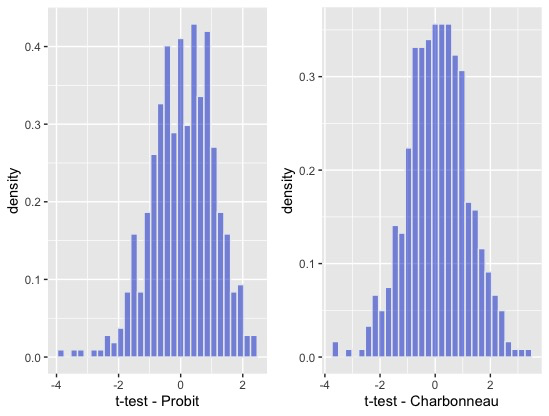
\includegraphics[scale=0.35]{content/Figures/ttest_beta21_Design6.png}}
        \caption{\footnotesize{Histogram of the \textit{t-test} for estimated $\beta_{21}^*$ in Design 6}}
        \label{ttest_beta21_Design6}
      \end{figure}
    Design that do not contain fixed effects in selection equation both approaches deliver similar results: distributions are centered around zero.
\end{frame}

\begin{frame}
    \frametitle{Simulations: First stage \textit{t-tests} for structural parameters}
    \begin{figure}
        \centerline{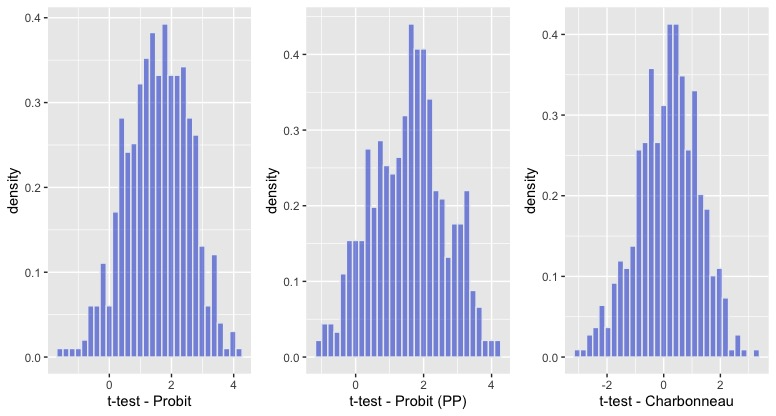
\includegraphics[scale=.35]{content/Figures/ttest_beta21_Design5.png}}
        \caption{\footnotesize{Histogram of the \textit{t-test} for estimated $\beta_{21}^*$ in Design 5}}
        \label{ttest_beta21_Design5}
      \end{figure}
\end{frame}

\begin{frame}
    \frametitle{Simulations: First stage \textit{t-tests} for structural parameters}
    \begin{figure}
        \centerline{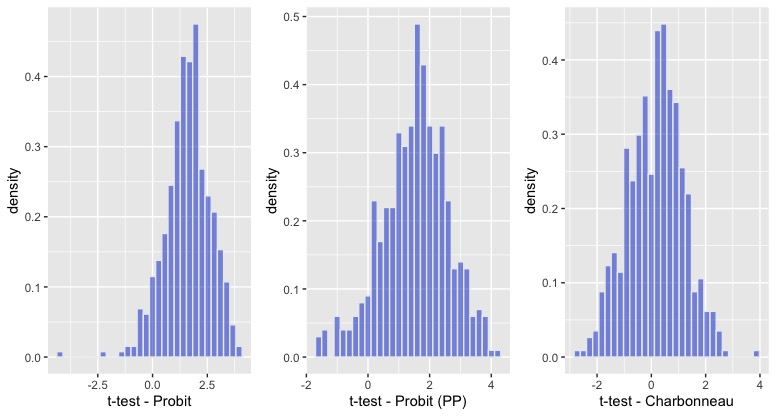
\includegraphics[scale=.35]{content/Figures/ttest_beta21_Design7.png}}
        \caption{\footnotesize{Histogram of the \textit{t-test} for estimated $\beta_{21}^*$ in Design 7}}
        \label{ttest_beta21_Design7}
      \end{figure}
      For Charbonneau, \textit{t-tests} are centered around zero, but not for Probit and Probit (PP). Biases of estimates for Probit and Probit (PP) are of the same magnitude $\xrightarrow{}$ reflects mostly incidental parameter problem.
\end{frame}

\begin{frame}
    \frametitle{Simulations: First stage QQ-plot for structural parameters}
    \begin{figure}
        \centerline{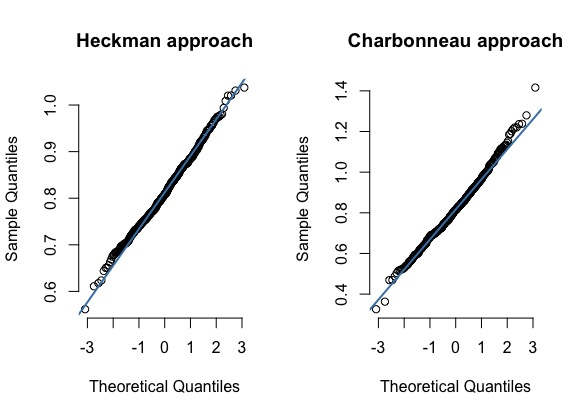
\includegraphics[scale=.35]{content/Figures/QQ_beta_21_Design6.png}}
        \caption{\footnotesize{QQ plot of estimated $\beta_{21}^*$ in Design 6}}
        \label{QQ_beta_21_Design6}
      \end{figure}
      All distributions are reasonably well approximated by a normal distribution.
\end{frame}

\begin{frame}
    \frametitle{Simulations: First stage QQ-plot for structural parameters}
    \begin{figure}
        \centerline{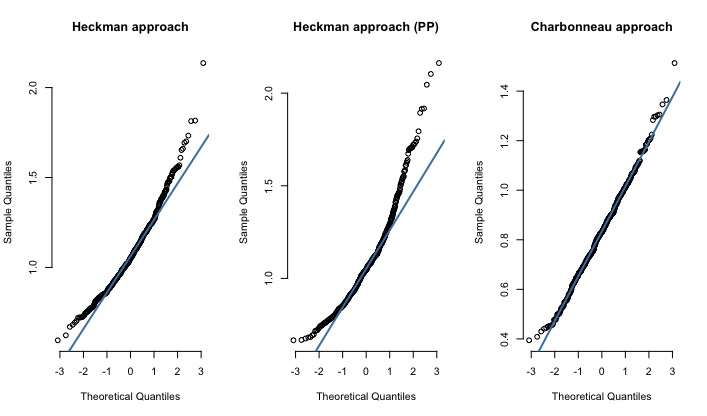
\includegraphics[scale=.35]{content/Figures/QQ_beta_21_Design5.png}}
        \caption{\footnotesize{QQ plot of estimated $\beta_{21}^*$ in Design 5}}
        \label{QQ_beta_21_Design5}
      \end{figure}
\end{frame}

\begin{frame}
    \frametitle{Simulations: First stage QQ-plot for structural parameters}
    \begin{figure}
        \centerline{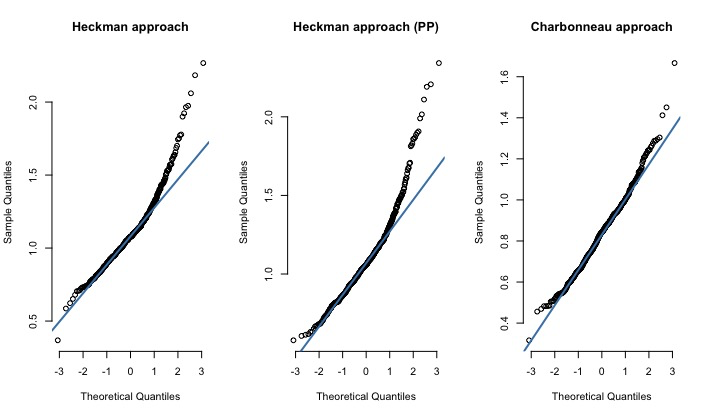
\includegraphics[scale=.35]{content/Figures/QQ_beta_21_Design7.png}}
        \caption{\footnotesize{QQ plot of estimated $\beta_{21}^*$ in Design 7}}
        \label{QQ_beta_21_Design7}
      \end{figure}
      In designs 5 and 7, Charbonneau are better approximated by a normal distribution. Other estimators are more skewed.
\end{frame}

\begin{frame}
    \frametitle{Simulations: First stage fixed effects}
    \begin{figure}
        \centerline{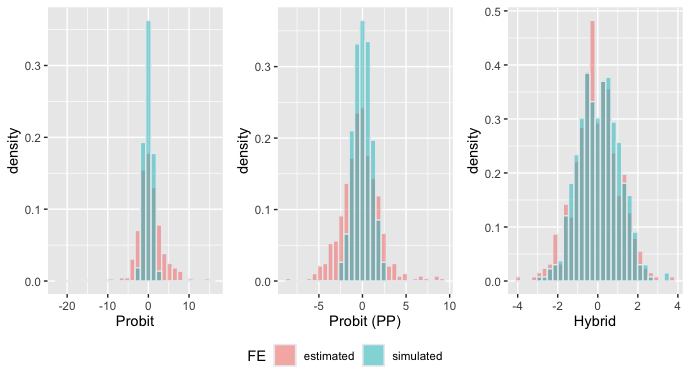
\includegraphics[scale=.35]{content/Figures/Hist_FE_Design5.png}}
        \caption{\footnotesize{Histogram of estimated $\xi_1^*$ in Design 5}}
        \label{fig}
      \end{figure}
\end{frame}

\begin{frame}
    \frametitle{Simulations: First stage fixed effects}
    \begin{figure}
        \centerline{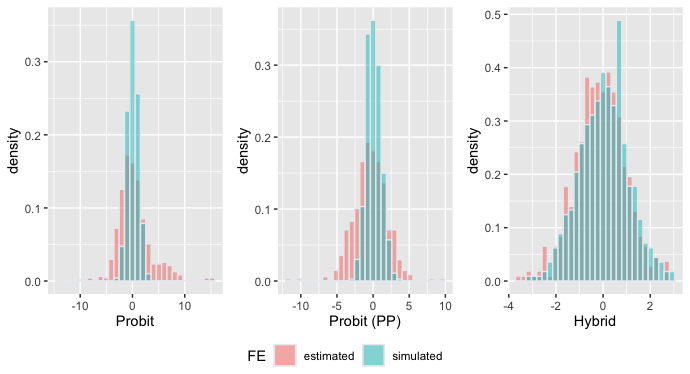
\includegraphics[scale=.35]{content/Figures/Hist_FE_Design7.png}}
        \caption{\footnotesize{Histogram of estimated $\xi_1^*$ in Design 7}}
        \label{fig}
      \end{figure}
      Probit estimates off due to: (i) not corrected for perfect prediction, and (ii) estimates are contaminated by the (asymptotic) bias of structural parameters.
      \hyperlink{single indices}{\beamerbutton{Results of single indices}}
\end{frame}

\begin{frame}
    \frametitle{Simulations: Second stage structural parameters mean bias}
    \begin{minipage}{7cm}
    \begin{figure}[htbp]
      \centerline{\includegraphics[scale=.28]{content/Figures/bias_beta11_design6.eps}}
      \caption{\footnotesize{Mean bias of  $\hat{\beta}_{11}$ in Design 6}}
      \label{bias_beta11_design6}
    \end{figure}
    \begin{figure}[htbp]
      \vspace{-2.5em}%
      \centerline{\includegraphics[scale=.28]{content/Figures/bias_beta12_design6.eps}}
      \caption{\footnotesize{Mean bias of  $\hat{\beta}_{12}$ in Design 6}}
      \label{bias_beta12_design6}
    \end{figure}
  \end{minipage}%
  \begin{minipage}{5cm}
             For the modified Kyriazidou: $r=1$ and $K$ set to be a standard normal density.\\~\\
             With no fixed effects, all proposed estimators have essentially no bias. \\~\\
             Even when including dummies in observation equations, estimators have nice properties. 
            \end{minipage}
  \end{frame}

  \begin{frame}
    \frametitle{Simulations: Second stage structural parameters mean bias}
    \begin{minipage}{7cm}
    \begin{figure}[htbp]
      \centerline{\includegraphics[scale=.28]{content/Figures/bias_beta11_design5.eps}}
      \caption{\footnotesize{Mean bias of  $\hat{\beta}_{11}$ in Design 5}}
      \label{bias_beta11_design5}
    \end{figure}
    \begin{figure}[htbp]
      \vspace{-2.5em}%
      \centerline{\includegraphics[scale=.28]{content/Figures/bias_beta12_design5.eps}}
      \caption{\footnotesize{Mean bias of  $\hat{\beta}_{12}$ in Design 5}}
      \label{bias_beta12_design5}
    \end{figure}
  \end{minipage}%
  \begin{minipage}{5cm}
    Heckman and Heckman(PP) have biases: single indices are biased.\\~\\
  \end{minipage}
  \end{frame}

  \begin{frame}
    \frametitle{Simulations: Second stage structural parameters mean bias}
    \begin{minipage}{7cm}
    \begin{figure}[htbp]
      \centerline{\includegraphics[scale=.28]{content/Figures/bias_beta11_design7.eps}}
      \caption{\footnotesize{Mean bias of  $\hat{\beta}_{11}$ in Design 7}}
      \label{bias_beta11_design7}
    \end{figure}
    \begin{figure}[htbp]
      \vspace{-2.5em}%
      \centerline{\includegraphics[scale=.28]{content/Figures/bias_beta12_design7.eps}}
      \caption{\footnotesize{Mean bias of  $\hat{\beta}_{12}$ in Design 7}}
      \label{bias_beta12_design7}
    \end{figure}
  \end{minipage}%
  \begin{minipage}{5cm}
    Kyriazidou reduces further the bias for the continuous variable.\\~\\
    Hybrid reduces further for the binary variable. \\~\\
    Estimates sensitive to initial choice of $h$.\\
    \hyperlink{qqplots}{\beamerbutton{QQ plots}}
  \end{minipage}
  \end{frame}




\section{Application to international trade flows}
\begin{frame}
    \frametitle{Application to gravity model: Selection Equation}
    \textbf{Aim:} estimate how trade barriers affect both the decision of country $i$ to export to country $j$, and the volume of trade. \pause
    \\~\\ 
    \textbf{Dataset:} provided by \cite{helpman2008estimating}. Information on directed trade flows and country characteristics for 158 countries in 1986. \\
    Exclude Congo as exporter: avoid the problem of perfect prediction. \pause
    \\~\\ 
    \textbf{First stage equation:} Same equation estimated by \cite{helpman2008estimating}.
    \begin{align*}
        y_{2,i j}= \mathbbm{1}(x_{2,ij}'\beta_2^* +\xi_{i}^*+\zeta_{j}^* >\eta_{i j}^*)
    \end{align*}
    
    \noindent where: \\
    (i) $y_{2,i j}$ is a binary variable, being one if the $i$ exports to $j$ and zero otherwise \\
    (ii) $\xi_{i}^*$ is the exporter fixed effect \\(iii) $\zeta_{j}^*$ is the importer fixed effect \\(iv) $x_{2,ij}$ is the vector that collects the variables \textit{Distance}$_{ij}$, \textit{Common Border}$_{ij}$, \textit{Colonial Ties}$_{ij}$, \textit{Currency Union}$_{ij}$, \textit{Common Legal System}$_{ij}$, \textit{FTA}$_{ij}$, \textit{Common Religion}$_{ij}$.
\end{frame}

\begin{frame}
    \frametitle{Application to gravity model: Selection Equation}
    \begin{table}
        \fontsize{8}{8}\selectfont
        \centering
        \begin{threeparttable}
        \captionsetup{font=scriptsize}
        \begin{tabular}{p{4cm}p{1.8cm}p{1.8cm}}
          \hline
          \\[-0.5em]
           \quad & Probit  & Charbonneau \\
           \\[-0.5em]
           \hline
           \\[-0.5em]
            \textit{Common Language}  &  $0.2903^{***}$ (0.0379) &  $0.4248^{***}$ (0.0732) \\
            \\[-0.5em]
            \textit{Common Legal System}  &  $0.0972^{**}$ (0.0296) &  $0.1822^{***}$ (0.0597)\\
            \\[-0.5em]
            \textit{Common Religion} & $0.2647^{***}$ (0.0585)&  $0.4979^{***}$ (0.1125)\\
            \\[-0.5em]
            \textit{Common Border} & $-0.3798^{***}$ (0.0946) &  $-0.5164^{**}$ (0.2300)\\
            \\[-0.5em]
            \textit{Currency Union} &  $0.4883^{***}$ (0.1306) &  $1.0459^{***}$ (0.2362)\\
            \\[-0.5em]
            \textit{Distance}  & $-0.6626^{***}$ (0.0208) &  $-1.0001^{***}$ (0.0541)\\
            \\[-0.5em]
            \textit{FTA} &  $2.0170^{***}$ (0.3085) & $3.5565^{***}$ (0.5237)\\
            \\[-0.5em]
            \textit{Colonial Ties} &  $0.3337$ (0.2852) &  $1.1432^{*}$ (0.6473)\\
             & &  \\
            \hline
        \end{tabular}
        \caption{{Estimates for the first stage. Standard errors are in parenthesis. \\
        \textsuperscript{*} indicates that the coefficient is significant at the 10 \% level \\
        \textsuperscript{**} indicates that it is significant at the 5 \% level \\ \textsuperscript{***} indicates that it is significant at the 1 \% level.}}
    \end{threeparttable}
        \label{tab:app1}
    \end{table}
\end{frame}

\begin{frame}
    \frametitle{Application to gravity model: Observation Equation}  
    \textbf{Second stage equation:} Difference to equation estimated by \cite{helpman2008estimating} is that we do not take into account $w_{ij}$.
    \begin{align*}
        y_{1,ij,t} = x_{1,ij,t}'\beta_1 + \vartheta_i + \chi_j + u_{ij,t}
    \end{align*}
    
    \noindent where: \\
    (i) $y_{1,ij}$ is the log of the value of the exports from $i$ to $j$ \\
    (ii) $\vartheta_i$ is the exporter fixed effect \\ (iii) $\chi_j$ is the importer fixed effect \\
    (iv) $x_{1,ij,t}$ is the vector that collects the same variables as $x_{2,ij}$, with the exception of \textit{Common Religion}$_{ij}$ (exclusion restriction) \\~\\ 
    \textbf{Equation estimated using only observations with positive trade flows $\xrightarrow{}$ sample selection correction needed.}
\end{frame}

\begin{frame}
    \frametitle{Application to gravity model: Observation Equation}  
    \begin{table}
        \fontsize{8}{8}\selectfont
        \captionsetup{font=scriptsize}
        \centering
        \begin{tabular}{p{2.6cm}p{1.4cm}p{1.4cm}p{1cm}p{1cm}p{1cm}p{1cm}}
          \hline
          \\[-0.5em]
           \quad  &Heckman (1) & Heckman (2) &Hybrid  & K (h=0.5)  & K (h=3)  & K (h=10)  \\
           \\[-0.5em]
           \hline
           \\[-0.5em]
            \textit{Common Language}  & $0.2090^{***}$ & $0.2333^{***}$& 0.3566 & 0.1094 & 0.1830& 0.1994\\
            \\[-0.5em]
            \textit{Legal System}  & $0.4797^{***}$ & $0.4914^{***}$& 0.4975 & 0.3805& 0.4206&0.4255\\
            \\[-0.5em]
            \textit{Common Border}  & $0.4031^{***}$ & $0.4318^{***}$ & 0.5836& 0.6114 &0.5673 & 0.5129\\
            \\[-0.5em]
            \textit{Currency Union}   & $1.3537^{***}$ & $1.3368^{***}$ & 1.4456 & 1.2315& 1.4164&1.4213\\
            \\[-0.5em]
            \textit{Distance}   & $-1.2087^{***}$ & $-1.2190^{***}$& -1.3470& -1.1371& -1.2503& -1.1721\\
            \\[-0.5em]
            \textit{FTA}  &  $0.7774^{***}$ & $0.7719^{***}$& 2.0569 & 1.2835& 1.2408& 0.2901\\
            \\[-0.5em]
            \textit{Colonial Ties}  & $1.3418^{***}$ & $1.3434^{***}$ & 1.4209 & 1.2594 & 1.3387 & 1.1945\\
            \\[-0.5em]
            \textit{Common Religion}  &  $0.2389^{**}$ &  &  &  &  & \\
            \\[-0.5em]
            \textit{Inverse Mills-Ratio}  & $0.2784^{***}$ & $0.2671^{***}$ & 0.7130& & & \\
             &  & & & & & \\
            \hline
        \end{tabular}
        \caption{\footnotesize{Estimates for the second stage equation. We denote by Kyriazidou by $K$. \newline \textsuperscript{*} indicates that the coefficient is significant at the 10 \% level \newline \textsuperscript{**} indicates that the coefficient is significant at the 5 \% level \newline \textsuperscript{***} indicates that the coefficient is significant at the 1 \% level.}}
        \label{tab:app2}
\end{table}
\end{frame}
\section{Conclusion}
\begin{frame}
    \frametitle{Conclusion}
    \begin{itemize}
        \item Accounting for sample selection in dyadic settings requires more involved methods than the standard \cite{heckman1979sample} approach.
        \item Difficulty arises through the incidental parameter problem in the selection equation.
        \item \cite{charbonneau2017multiple} estimator:
        \begin{itemize}
            \item Leads to estimates that are free of this problem in the first stage.
            \item However, it does not deliver estimates of fixed effects essential to employ Heckman approach.
        \end{itemize}
        \item To bypass this problem, we proposed:
        \begin{itemize}
            \item To get the FE through a Hybrid estimation and further apply the Heckman procedure after a transformation is made in the selection equation. \\
            $\xrightarrow{}$ it may not be well suited for sparse networks
            \item A modification to the \cite{kyriazidou1997estimation} estimator. \\
            $\xrightarrow{}$ no need for FE estimates.\\
            $\xrightarrow{}$ estimates are sensitive to chosen bandwidth. \\
            $\xrightarrow{}$ needs a variable that satisfies exclusion restriction
        \end{itemize} 
        \item Drawbacks: computational costs!
        \item Simulations confirm the theoretical predictions that biases are reduced.
    \end{itemize}
\end{frame}

\appendix
\begin{frame}[allowframebreaks]
  \frametitle{References}
  \bibliographystyle{plainnat}
  \bibliography{library.bib}
\end{frame}
\begin{frame}[label=Gravity model]
    \frametitle{Gravity model of \cite{helpman2008estimating} : Features}
    \begin{block}{Definition}
        Multilateral resistance term: country's average trade barrier with all its trading partners (\cite{anderson2003gravity}).
    \end{block} 
    Two main features:
    \begin{itemize}
        \item Multilateral resistance terms.
        \item Theoretical framework that takes into account sample selection. 
        \begin{itemize}
            \item A fraction of firms in country $i$ decides to export to country $j$. 
            \item Firms have individual heterogeneous productivity and face variable and fixed costs when exporting.
        \end{itemize}
    \end{itemize}
  \end{frame}
  \begin{frame}
    \frametitle{Gravity model of \cite{helpman2008estimating}}
    Considering that:
    \begin{enumerate}
        \item Country $i$ has $N_i$ heterogeneous firms.
        \item Productivity is firm-specific given by $\frac{1}{a}$, $a$ follows a cumulative distribution function $G(a)$, with support $[a_L, a_H]$.
        \item Firm in country $i$ has input costs $c_ia$ per unit of output.
        \item If it sells in country $j$, it incurs:
        \begin{itemize}
            \item Fixed costs $c_i f_{ij}$.
            \item Variable costs (melting iceberg): $\tau_{ij}$ units of a product needs to be shipped from country $i$ to $j$ for one unit to arrive.
        \end{itemize} 
        \item CES preferences.
        \item Products are differentiated according to country of origin.
        \item Monopolistic competition in the final products.
        \item Economy of $I$ countries indexed by $i=1,...I$
    \end{enumerate}
  \end{frame}
  
  \begin{frame}
    \frametitle{Gravity model of \cite{helpman2008estimating}}
    Model delivers the system of equations:
    \begin{align}
        (1-\alpha)\left(\frac{\tau_{i j} c_{i} a_{i j}}{\alpha P_{j}}\right)^{1-\sigma} Y_{j}=c_{i} f_{i j}
        \label{eq:MHR1}
    \end{align}
    \noindent where : $a_{ij}$ is defined as the point where profits are exactly zero, $P_j$ the price index of the economy of country $j$, $Y_j$ the size of its economy and $\sigma = 1/(1-\alpha)$ is the elasticity of substitution across products. 
    \\~\\
    The fraction of country $i$'s $N_i$ firms that export to country $j$, is given by $G(a_{ij})$.
  \end{frame}

  \begin{frame}
    \frametitle{Gravity model of \cite{helpman2008estimating}}
    \begin{align}
        V_{i j}=\left\{\begin{array}{cc}
    \int_{a_{L}}^{a_{i j}} a^{1-\sigma} d G(a) & \text { for } a_{i j} \geq a_{L} \\
    0 & \text { otherwise }
    \end{array}\right.
    \label{eq:MHR2}
    \end{align}
    \noindent where $V_{ij}$ determines the bilateral trade volume. 
    \begin{align}
        Y_{1,i j}=\left(\frac{c_{i} \tau_{i j}}{\alpha P_{j}}\right)^{1-\sigma} Y_{j} N_{i} V_{i j}
        \label{eq:MHR3}
    \end{align}
    defines the value of country $j$'s imports from $i$ ($Y_{1,ij}$). 
    \begin{align} \label{eq:MHR4}
        P_{j}^{1-\sigma}=\sum_{i=1}^{I}\left(\frac{c_{i} \tau_{i j}}{\alpha}\right)^{1-\sigma} N_{i} V_{i j}
    \end{align}
    defines the price indices of country $j$.
  \end{frame}

  \begin{frame}
    \frametitle{Estimation method of \cite{helpman2008estimating}}
    \begin{block}{Assumption 1:}
      Firm productivity $\frac{1}{a}$ is Pareto distributed, with support $[a_L,a_H]$.
    \end{block} 
    \begin{block}{Assumption 2:}
        There are i.i.d. unmeasured country-pair specific trade frictions $u_{ij,t} \sim N(0, \sigma_u^2)$ such that: $\tau_{i j,t}^{\sigma-1} \equiv D_{i j,t}^{\gamma} e^{-u_{i j,t}} $ \\
    where $D_{ij,t}$ is the symmetric distance between $i$ and $j$. 
      \end{block} 
      \begin{block}{Assumption 3:}
        There are i.i.d. unmeasured country-pair specific trade frictions $\nu_{ij,t}\sim N(0, \sigma_\nu^2)$ that may be correlated with $u_{ij,t}$, such that: $f_{i j,t} \equiv \exp \left(\phi_{E X, i}+\phi_{I M, j}+\kappa \phi_{i j,t}-\nu_{i j,t}\right)$ \\
        where $\phi_{I M, j}$ is a fixed trade barrier imposed by the importing country, $\phi_{E X, i}$ is a measure of fixed export costs, and $\phi_{i j,t}$ is an observed measure of country-pair specific fixed trade costs.
      \end{block} 
  \end{frame}

  \begin{frame}
    \frametitle{Estimation method of \cite{helpman2008estimating}}
    Given Assumptions 1, 2 and 3, and by log-linearizing the gravity equation, which defines the export volume from country $i$ to $j$:
\begin{align}
    y_{1,ij,t} = x_{1,ij,t}'\beta_1 + \vartheta_i + \chi_j + w_{ij,t} + u_{ij,t},
    \label{eq:est_MHR_wage}
\end{align}

\noindent where: \\
(i) $y_{1,ij,t} = \ln Y_{1,ij,t}$ \\
(ii) $w_{ij,t} = \ln W_{ij,t}$ \\
(iii) $\beta_1$ is a vector that collects the coefficients of the remaining structural parameters, $\beta_1 = (\beta_0, \gamma_1')'$\\
(iv) $x_{1,ij,t}$ is a vector that collects 1 and the vector $ d_{ij,t} = \ln D_{ij,t}$\\
(v) $\chi_j = (\sigma -1) \ln P_j + \ln Y_j$, which is an importer fixed effects\\
(vi) $\vartheta_i = -(\sigma - 1) \ln c_i + \ln N_i$, which is an exporter fixed effects.
\\~\\
Important difference to the equation derived in previous studies: the new variable $w_{ij,t}$, which controls for the fraction of firms exporting. 
  \end{frame}

  \begin{frame}
    \frametitle{Estimation method of \cite{helpman2008estimating}}
    Latent variable $Y_{2,ij,t}^*$ is given by the ratio of variable export profits for the most productive firm (with productivity $1/a_L$) to the fixed export costs for exports from $i$ to $j$ (expressions that are given by the zero profit condition). Then, in this case, positive exports are observed if $Y_{2,ij,t}^* > 1$.\\~\\
    
    By log-linearizing the equation for the latent variable $Y_{2,ij,t}^*$, and given Assumption 3, we have that:
\begin{align}
    y_{2,i j,t}^*= x_{2,ij,t}'\beta_2 +\xi_{i}+\zeta_{j} +\eta_{i j,t},
    \label{eq:est_MHR_sampleselection}
\end{align}

\noindent where: \\
(i) $\eta_{ij,t} \equiv u_{ij,t} + \nu_{ij,t} \sim N(0, \sigma_u^2 + \sigma_\nu^2)$ is i.i.d., but correlated with $u_{ij,t}$ \\
 (ii) $\xi_{i}=-\sigma \ln c_{i}+\phi_{E X, i}$ is an exporter fixed effect \\
 (iii) $\zeta_{j}=(\sigma-1) \ln P_{j}+ \ln Y_{j}-\phi_{I M, j}$ is an importer fixed effect\\
  (iv) $\beta_2$ is a vector that collects the coefficients of the remaining structural parameters, $\beta_2 = (\gamma_0, \gamma_2')'$ \\
   (iv) $x_{2,ij,t}$ is a vector that collects 1, and the vectors $ d_{ij,t} = \ln D_{ij,t}$, and $\phi_{ij,t}$.
   \\~\\
    $x_{2,ij,t}$ includes both the regressors in $x_{1,ij,t}$ and additional regressors that affect only the decision to export, but not the volume of exports (exclusion restriction). 
  \end{frame}
\begin{frame}[label = Heckman]
    \frametitle{The Heckman's steps}
    The least squares estimators of $\beta_1$ and $\sigma_{u\eta^*}$ are unbiased but inefficient, due to the heteroskedasticity in $\mathbbm{E}[\nu_{ij,t}^2]$, as shown in \cite{heckman1979sample}:
\begin{align*}
    \mathbbm{E}[\nu_{ij,t}^2] = \sigma_u^2 \Big((1-\rho^2) + \rho^2(1+ z_{ij,t} \lambda_{ij,t} - \lambda_{ij,t}^2)\Big)
\end{align*}

\begin{itemize}
    \item Step 1: Estimate the probability that $y^{**}_{2,ij,t} \geq 0$ using probit analysis on the sample, given by the selection equation.
    \item Step 2: From this estimator (provided that it is consistent), one can obtain $\hat{z}_{ij,t}$ consistently.
    \item Step 3: The estimated value of $\lambda_{ij,t}(z_{ij,t})$ is used as a regressor in the observation equation fit on the subsample. The regression estimators are then consistent for $\beta_1$ and $\sigma_{u\eta^*}$.
    \item Step 4: One can then consistently estimate $\sigma_u^2$ from the following. From step (3), we consistently estimate $\sigma_{u\eta^*}$, through the estimator $\hat{\sigma}_{u\eta^*}$. Denote the residuals for each observation from step 3 as $\hat{\nu}_{ij,t}$. Then, using $\hat{z}_{ij,t}$ and $\hat{\lambda}_{ij,t}$ the estimated values from step (2), an estimator of  $\sigma_u^2$ is:
    $$\hat{\sigma}_u^2 = \frac{\sum_{i=1}^{N_i}\sum_{j\neq i}\sum_{t=1}^T \hat{\nu}_{ij,t}^2}{N_i(N_i-1)T} - \frac{\hat{\sigma}_{u\eta^*}}{N_i(N_i-1)T}  \sum_{i=1}^{N_i}\sum_{j\neq i}\sum_{t=1}^T (\hat{\lambda}_{ij,t} \hat{z}_{ij,t} - \hat{\lambda}_{ij,t}^2)$$
\end{itemize}

\end{frame}
\begin{frame}[label = Asymptotic]
    \frametitle{Incidental parameter problem}
    \cite{heckman1979sample}'s approach:
    \begin{itemize}
        \item \textbf{Stage 1:} Estimate the selection equation by MLE (probit).
        \item \textbf{Stage 2:} Obtain inverse Mills-ratio and estimate the observation equation by FGLS.
    \end{itemize} 
    \textbf{But} fixed effects estimators in nonlinear models suffer from the \textbf{incidental parameter problem} (\cite{neyman1948consistent}). 
    \\~\\
    \textbf{How does this problem arise?}\\
    $y_{2,ij,t}$ is generated by the process:
\begin{align*}
    y_{2,ij,t} \rvert x_{2,ij,t}, \xi^*, \zeta^*, \beta_2^* \sim f_{Y_2}(\cdot \rvert x_{2,ij,t}, \xi^*, \zeta^*, \beta_2^*)
\end{align*}
\noindent where: $\xi^* = (\xi_1^*, ... \xi_N^*)$, $\zeta^* = (\zeta_1^*, ... \zeta_N^*)$, $f_{Y_2}$ is a known probability function and $\xi^*_i, \zeta^*_j$ are the unobserved fixed effects.
\end{frame}

\begin{frame}
    \frametitle{Incidental parameter problem}
Using a single-index specification with fixed effects:
\begin{align}
    f_{Y_2} ( y_{2,ij,t} \rvert  x_{2,ij,t}, \xi^*, \zeta^*, \beta_2^*) &= \Phi(x_{2,ij,t}'{\beta_2^*}  +\xi_{i}^*+\zeta_{j}^*)^{y_{2,ij,t}} \nonumber\\ 
    &\times [1 - \Phi(x_{2,ij,t}'{\beta_2^*}  +\xi_{i}^*+\zeta_{j}^*)]^{1-y_{2,ij,t}}, 
    \label{eq:fy}
 \end{align}
 To estimate the parameters, we solve the sample analogue of:
\begin{align}
    \max_{(\beta_2^*, \omega_{NN}^*) \in \mathbb{R}^{\text{dim} \beta_2^* + \text{dim} \omega_{NN}^*}} \mathcal{L} (\beta_2^*, \omega_{NN}^*)
    \label{eq:val1}
\end{align}
\noindent with $\omega_{NN}^* = {(\xi_1^*, ... \xi_N^*, \zeta_1^*, ... \zeta_N^*)}'$, and:
\begin{align} \label{eq:unconditional}
    &\mathcal{L} (\beta_2^*, \omega_{NN}^*) \\ &= (N(N-1)T)^{-1} \Big\{ \sum_{i=1}^{N}\sum_{j\neq i}\sum_{t=1}^T \log f_{Y_2} ( y_{2,ij,t} \rvert  x_{2,ij,t}, \xi^*, \zeta^*, \beta_2^*) - b(\iota'_{NN} \omega_{NN}^*)^2/2 \Big\} \nonumber
\end{align}
\noindent $b>0$ is an arbitrary constant, $\iota_{NN} = (1_N', - 1_N')'$ and $1_N$ denotes a vector of ones of dimension $N$.
\end{frame}

\begin{frame}
    \frametitle{Incidental parameter problem}
For a given $\beta_2^*$, the optimal $\hat{\omega}_{NN}^*$ is:
\begin{align}
    \hat{\omega}_{NN}^*(\beta_2^*) = \argmax_{\omega_{NN}^* \in \mathbb{R}^{\text{dim} \omega_{NN}^*}} \mathcal{L} (\beta_2^*, \omega_{NN}^*)   
\end{align}
Then, the fixed effects estimator of $\beta_2^*$ and $\omega_{NN}^*$ are:
\begin{align} \label{eq:taylor}
    \hat{\beta}_2^* = \argmax_{\beta_2^* \in \mathbb{R}^{\text{dim} \beta_2^*}} \mathcal{L} (\beta_2^*, \hat{\omega}_{NN}^*(\beta_2^*))
 \end{align}
 \begin{align} \label{eq:omega}
     \hat{\omega}_{NN}^*(\beta_2^*) = \hat{\omega}_{NN}^*(\hat{\beta}_2^*)
 \end{align} 
 \textbf{The source of the problem is that the dimension of the nuisance parameters increase with sample size and their estimation converge at a slower rate than the structural parameters.}
\end{frame}

\begin{frame}
    \frametitle{Incidental parameter problem}
    Denote:
    $$\Bar{\beta}^*_2 = \argmax_{\beta^*_2 \in \mathbb{R}^{\text{dim} \beta^*_2}} \mathbb{E}_\omega \Big[\mathcal{L} (\beta^*_2, \hat{\omega}_{NN}^*(\beta^*_2)) \Big]$$
    Using an asymptotic expansion for smooth likelihoods under appropriate regularity conditions (\cite{fernandez2016individual}):
    \begin{align} \label{eq:val2}
        \Bar{\beta}_2^* = \beta_{2,0}^* + \frac{\Bar{B}_\infty}{(N-1)T} + \frac{\Bar{D}_\infty}{(N-1)T} + \text{o}_P(((N-1)T)^{-1})
    \end{align}
    For some constants $\Bar{B}_\infty$ and $\Bar{D}_\infty$. 
    By the properties of the maximum likelihood estimator:
    \begin{align}
        \sqrt{N(N-1)T} (\hat{\beta}_2^* - \Bar{\beta}_2^*) \xrightarrow{d} N(0, \Bar{V_B}_\infty)
    \end{align}
    For some $\Bar{V_B}_\infty$. By Slutsky Theorem:
    \begin{align} \label{eq:val3}
        \sqrt{N(N-1)T} (\hat{\beta}_2^* - \beta_{2,0}^*) \xrightarrow{d} N\Big( \frac{\Bar{B}_\infty}{\sqrt{T}} + \frac{\Bar{D}_\infty}{\sqrt{T}}, \Bar{V_B}_\infty\Big) \nonumber
    \end{align}
\end{frame}

\begin{frame}
    \frametitle{Incidental parameter problem: asymptotic expansion}
    Taking a first-order Taylor expansion of the first order conditions of Equation (\ref{eq:taylor}) around $\beta_{2,0}^*$, gives:
    \begin{align} 
     0 &= \frac{\partial \mathcal{L} (\hat{\beta}_2^*, \hat{\omega}_{NN}^*(\beta_2^*))}{\partial_{\beta_2^*}}  \approx \frac{\partial \mathcal{L} ({\beta}_{2,0}^*, \hat{\omega}_{NN}^*(\beta_{2,0}^*))}{\partial_{\beta_2^*}} \nonumber \\
     &- \Bar{W}_\infty \sqrt{N(N-1)T} (\hat{\beta}_2^* - \beta_{2,0}^*)
    \end{align}
    
    Then, we apply a second-order Taylor expansion to approximate the above term $\frac{\partial  \mathcal{L} ({\beta}_{2,0}^*, \hat{\omega}_{NN}^*(\beta_{2,0}^*))}{\partial_{\beta_2^*}}$ around $\omega_{NN}^*(\beta_{2,0}^*)$, such that the estimates of the fixed effects are taken into account.
    \begin{align}
        &\frac{\partial \mathcal{L} ({\beta}_{2,0}^*, \hat{\omega}_{NN}^*(\beta_{2,0}^*))}{\partial_{\beta_{2}^*}}  \approx \frac{\partial \mathcal{L} ({\beta}_{2,0}^*, {\omega}_{NN}^*(\beta_{2,0}^*))}{\partial_{\beta_{2}^*} } \\
        &+ \frac{\partial^2 \mathcal{L} ({\beta}_{2,0}^*, {\omega}_{NN}^*(\beta_{2,0}^*)) }{\partial_{\beta_{2}^*} \partial_{\omega_{NN}'} }[ \hat{\omega}_{NN}^* (\beta_{2,0}^*) - \omega_{NN}^* (\beta_{2,0}^*)]  \nonumber\\
        &+ \sum_{k = 1}^{\text{dim } \omega_{NN}} \frac{\partial^3 \mathcal{L} ({\beta}_{2,0}^*, {\omega}_{NN}^*(\beta_{2,0}^*))}{\partial_{\beta_{2}^*} \partial_{\omega_{NN}'} \partial_{\omega_{NN,k}}}[ \hat{\omega}_{NN}^* (\beta_{2,0}^*) - \omega_{NN}^* (\beta_{2,0}^*)] [ \hat{\omega}_{NN,k}^* (\beta_{2,0}^*) - \omega_{NN,k}^* (\beta_{2,0}^*)] / 2 \nonumber
    \end{align}
\end{frame}
    
\begin{frame}
        \frametitle{Incidental parameter problem: asymptotic expansion}
    Under regularity conditions, since the first term in this expression is the score vector, it has mean zero and it generates the asymptotic variance. By the information matrix equality and the Central Limit Theorem, we have:
    \begin{align} \label{eq:exp_1}
        \frac{\partial \mathcal{L} ({\beta}_{2,0}^*, {\omega}_{NN}^*(\beta_{2,0}^*))}{\partial_{\beta_{2}^*} }  \xrightarrow{d} N(0, \bar{W}_\infty)
    \end{align}
    
    For some variance $\bar{W}_\infty$. According \cite{fernandez2016individual}, the second and the third term satisfies:
    \begin{align} \label{eq:exp_2}
        &\frac{\partial^2 \mathcal{L} ({\beta}_{2,0}^*, {\omega}_{NN}^*(\beta_{2,0}^*)) }{\partial_{\beta_{2}^*}\partial_{\omega_{NN}'} }[ \hat{\omega}_{NN}^* (\beta_{2,0}^*) - \omega_{NN}^* (\beta_{2,0}^*)]  \nonumber\\
        &+ \sum_{k = 1}^{\text{dim } \omega_{NN}} \frac{\partial^3 \mathcal{L} ({\beta}_{2,0}^*, {\omega}_{NN}^*(\beta_{2,0}^*))}{\partial_{\beta_{2}^*}\partial_{\omega_{NN}'}\partial_{\omega_{NN,k}}}[ \hat{\omega}_{NN}^* (\beta_{2,0}^*) - \omega_{NN}^* (\beta_{2,0}^*)] [ \hat{\omega}_{NN,k}^* (\beta_{2,0}^*) - \omega_{NN,k}^* (\beta_{2,0}^*)] / 2 \nonumber \\
        & \approx \sqrt{N(N-1)T} \Big( \frac{\bar{B}^\beta_\infty}{(N-1)T} + \frac{\bar{D}^\beta_\infty}{(N-1)T} \Big)
    \end{align}
\end{frame}

\begin{frame}
        \frametitle{Incidental parameter problem: asymptotic expansion}
    The analytical form of terms $\bar{B}^\beta_\infty$ and $\bar{D}^\beta_\infty$ can be obtained from the second-order Taylor expansion as shown in \cite{fernandez2016individual}. Those terms originate from elements corresponding to the two-way fixed effects.
    
    Plugging in the expression (\ref{eq:exp_2}) into the equation for the first-order Taylor expansion, we have, as $N \xrightarrow{} \infty$:
    \begin{align}
        \Bar{W}_\infty \sqrt{N(N-1)T} (\hat{\beta}_2^* - \beta_{2,0}^*) = \frac{\partial \mathcal{L} ({\beta}_{2,0}^*, {\omega}_{NN}^*(\beta_{2,0}^*))}{\partial_{\beta_{2}^*} }  + \frac{\bar{B}^\beta_\infty}{\sqrt{T}} + \frac{\bar{D}^\beta_\infty}{\sqrt{T}} 
    \end{align}
    
    By Slutsky Theorem, we have, given (\ref{eq:exp_1}):
    \begin{align}
        \sqrt{N(N-1)T} (\hat{\beta}_2^* - \beta_{2,0}^*) \xrightarrow{d} \Bar{W}_\infty^{-1} N \Big(\frac{\bar{B}^\beta_\infty}{\sqrt{T}} + \frac{\bar{D}^\beta_\infty}{\sqrt{T}} , \Bar{W}_\infty \Big)
    \end{align}
    
    Therefore, compared to the expression given in the presentation, we have that:
    $$ \Bar{W}_\infty^{-1} \bar{B}^\beta_\infty = \bar{B}_\infty  $$
    $$ \Bar{W}_\infty^{-1} \bar{D}^\beta_\infty =  \bar{D}_\infty  $$
    
\end{frame}

\begin{frame}[label = Jochmans]
    \frametitle{{Conditional logit estimation: Estimator}}
    Denote: 
    \begin{itemize}
        \item $m_n$ distinct quadruples in the dataset. 
        \item a function $\sigma$ that maps the possible quadruples to an index set $N_{m_n} = \{ 1,2,...,m_n\}$. \\~\\ 
    \end{itemize} 
    Define the variables:
    \begin{align*}
        &z(\sigma\{l,i;j,k\}) = \frac{(y_{2,lj} - y_{2,lk}) - (y_{2,ij} - y_{2,ik})}{2} \\
        &r(\sigma\{l,i;j,k\}) = (x_{2,lj} - x_{2,lk}) - (x_{2,ij} - x_{2,ik}))
    \end{align*}
    Event that $z \in \{-1,1\}$ corresponds to the condition that for any $ij$, $l$ and $k$ satisfies $ y_{2,lk} + y_{2,lj} = 1, y_{2,ij} + y_{2,ik} = 1, y_{2,ij} + y_{2,lj} = 1$. \\~\\ 
    \textbf{Conditional on $x_2$ and $z \in \{-1,1\}$, the distribution of $z$ is logistic and does not depend on the fixed effects.}
    \begin{itemize}
        \item When $z=1$, we have necessarily that $y_{2,lk} = 1$, and when $z=-1$, it is necessarily zero.
    \end{itemize}
\end{frame}

\begin{frame}
    \frametitle{{Conditional logit estimation: Estimator}}
    The estimator is given by:
    \begin{align*}
        \hat{\beta}_2^* = \argmax_{\beta_2^* \in \Theta} \mathcal{L}_{CL}(\beta_2^*)
    \end{align*}
    \noindent $\Theta$ refers to the parameter space searched over, and $\mathcal{L}_{CL}$ is the objective function given by:
\begin{align*}
    \mathcal{L}_{CL}(\beta_2^*) &= \sum_{\sigma \in N_{m_n}} \mathbbm{1}\{ z(\sigma\{l,i;j,k\}) = 1\} \log (F(r(\sigma\{l,i;j,k\})'\beta_2^*)) \\ &+ \mathbbm{1}\{ z(\sigma\{l,i;j,k\}) = -1\} \log (1 - F(r(\sigma\{l,i;j,k\})'\beta_2^*))
\end{align*}  \\~\\ 
Denote:
\begin{itemize}
    \item $m_n^*$ the number of quadruples that contributes to the likelihood.
    \item $p_n$ the expected fraction of such quadruples over the total quadruples.
\end{itemize}
\end{frame}

\begin{frame}
    \frametitle{{Conditional logit estimation: Asymptotic Properties}}
    \begin{block}{Assumption 9:}
        $\beta_{2,0}^*$ is interior to $\Theta$, which is a compact subset of $\mathbbm{R}^{\text{dim} \beta_2^*}$.
    \end{block}
    
    \begin{block}{Assumption 10:}
        For all $(i,j) \in N \times N, \mathbbm{E}(\rvert \rvert x_{2,ij} \rvert \rvert^2) < c$, where $c$ is a finite constant.
    \end{block}
    
    \begin{block}{Assumption 11:}
        $Np_n \xrightarrow{} \infty$ as $N \xrightarrow{} \infty$ and the matrix
        $$ \lim_{N \xrightarrow{} \infty} (m_n p_n)^{-1} \sum_{\sigma \in N_{m_n}} \mathbbm{E} (r(\sigma\{l,i;j,k\}) r(\sigma\{l,i;j,k\})' f(r(\sigma\{l,i;j,k\})' \beta_{2,0}^*) \mathbbm{1}\{ z \in \{-1,1\}\}) $$
        has maximal rank, where $f$ is the density of the logistic function.
    \end{block} 

    \begin{block}{Theorem 2:}
        Let Assumptions 8 - 11 hold. Then, $\hat{\beta}_2^* \xrightarrow{p} \beta_{2,0}^*$ as $N \xrightarrow{} \infty$.
    \end{block}
\end{frame}

\begin{frame}
    \frametitle{{Conditional logit estimation: Asymptotic Properties}}
    To establish the limiting distribution, a stronger form of Assumption 10 is made, Then, as $N \xrightarrow{} \infty$:
    \begin{block}{Theorem 3:}
        Let Assumptions 8 - 12 hold. Then $\rvert \rvert \hat{\beta}_2^* - \beta_{2,0}^* \rvert \rvert = O_p (1/ \sqrt{N(N-1)p_n})$ and
        $$\Omega^{-1/2} (\hat{\beta}_2^* - \beta_{2,0}^*) \xrightarrow[]{d} N(0,I)$$
    \end{block}
    where:
    \begin{align*}
        &s(\sigma; \beta_2^*) = r_\sigma \{ \mathbbm{1} \{ z_\sigma = 1\} (1 - F({r_\sigma}' \beta_2^*)) - \mathbbm{1} \{ z_\sigma = - 1\}  F({r_\sigma}' \beta_2^*)\}, \\
    &\upsilon_{ij} (\beta_2^*) = \sum_{i \neq l,j} \sum_{k \neq i,l,j} s(\sigma\{l,i;j,k\}; \beta_2^*) \quad \quad \Upsilon (\beta_2^*) = \sum_{l=1}^N \sum_{j \neq l}  \upsilon_{ij} \upsilon_{ij}' \\
        &H (\beta_2^*) = \frac{\partial^2 \mathcal{L}_{CL}(\beta_2^*)}{\partial \beta_2^* \partial {\beta_2^*}'} = \sum_{\sigma \in N_{m_n}} r_\sigma r_\sigma' f(r_\sigma' \beta_2^*) \mathbbm{1}\{ z \in \{-1,1\}\} \\
        &\Omega = H {(\hat{\beta}_2^*)}^{-1} \Upsilon (\hat{\beta}_2^*) H {(\hat{\beta}_2^*)}^{-1}
\end{align*}
\end{frame}

\begin{frame}[label = h choice]
    \frametitle{Second approach: Choice of bandwidth}
    For a given order of differentiability $r$ of the expression $\mathbbm{E}(\Delta x_1' \bm{\varphi} \Phi \rvert \Delta x_2'\beta_2^*)$ and a given sample size $N(N-1)$, $h_n=h (N(N-1))^{-\mu}$ should be chosen such that $\mu = 1/(2 (r+1) +1)$. 
    \\~\\ 
    Value for $\mu$ comes from:
    \begin{itemize}
        \item Rate of convergence of the distribution of $\hat{\beta}_1$ is maximized by setting $\mu$ as small as possible.
        \item $\mu$ should be in the range $1-2p < \mu < p/2$, where $p$ is the rate of convergence of $\hat{\beta}_2^*$.
        \item  $\hat{\beta}_2^*$ should  converge fast enough: at least at a rate $p> (r+1)/(2(r+1)+1)$. \\~\\
    \end{itemize}  
    \textbf{Problem of choosing a bandwith boils down to choosing a constant $h$.} \\
    \cite{kyriazidou1997estimation}: for any positive initially chosen $h$, the distance between the estimator and the parameters' true values is minimized through a correction.
\end{frame}

\begin{frame}
    \frametitle{Second approach: Choice of bandwidth}
    \begin{block}{Corollary 1:}
        Let $\hat{\beta}_1$ be the estimator with window width $h_n = h  (N(N-1))^{-1/(2 (r+1) +1)}$, and $\hat{\beta}_{1,\delta}$ the estimator with window width $h_{n,\delta} = h  (N(N-1))^{-\delta/(2 (r+1) +1)}$ where $\delta \in (0,1)$. \\
        Define:
         $$\hat{\hat{\beta}}_1 = \frac{\hat{\beta}_1 - N(N-1)^{-(1-\delta)(r+1)/(2(r+1)+1)} \hat{\beta}_{1,\delta}}{1 - N(N-1)^{-(1-\delta)(r+1)/(2(r+1)+1)}}$$
         Then, $(\hat{\hat{\beta}}_1 - \beta_1)$ will converge to a normal distribution centered around 0 at rate $(N(N-1))^{-(r+1)/(2(r+1)-1)}$.
    \end{block}
    \textbf{Given an appropriately chosen $h_n$, using an estimated value for $\beta_2^*$ does not affect the limiting distribution of the estimator for $\beta_1$.}
\end{frame}

\begin{frame}[label = single indices]
    \frametitle{Simulation: single indices}
    \begin{figure}[htbp]
        \centerline{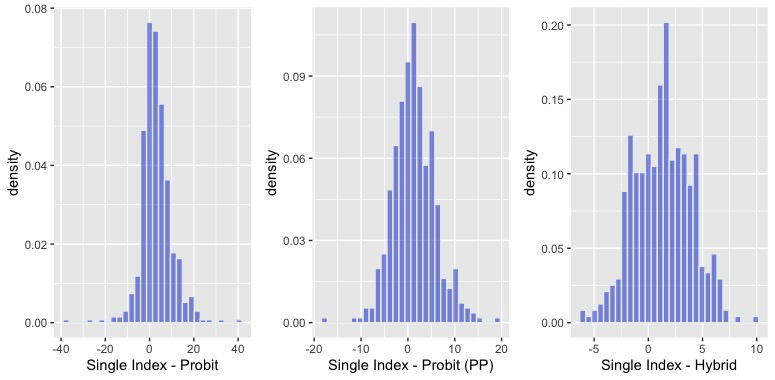
\includegraphics[scale=.35]{content/Figures/Hist_Zij_Design5.png}}
        \caption{\footnotesize{Histogram of $\hat{z}_{12} - z_{12}$ in Design 5}}
        \label{Hist_Zij_Design5}
      \end{figure}
\end{frame}

\begin{frame}
    \frametitle{Simulation: single indices}
    \begin{figure}[htbp]
        \centerline{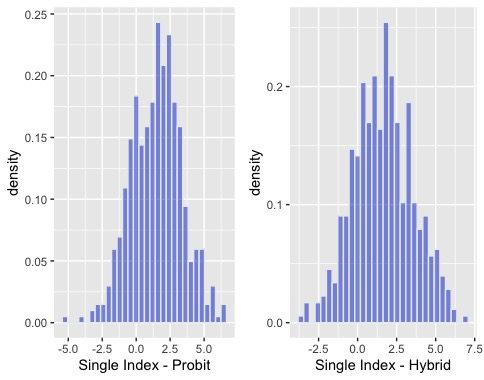
\includegraphics[scale=.35]{content/Figures/Hist_Zij_Design6.png}}
        \caption{\footnotesize{Histogram of $\hat{z}_{12} - z_{12}$ in Design 6}}
        \label{Hist_Zij_Design6}
      \end{figure}
\end{frame}

\begin{frame}
    \frametitle{Simulation: single indices}
    \begin{figure}[htbp]
        \centerline{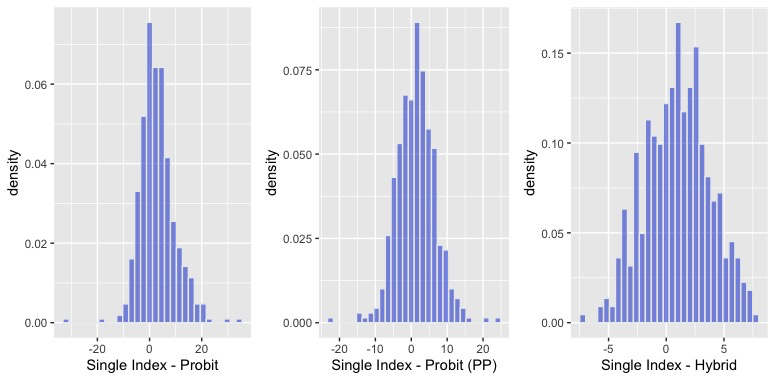
\includegraphics[scale=.35]{content/Figures/Hist_Zij_Design7.png}}
        \caption{\footnotesize{Histogram of $\hat{z}_{12} - z_{12}$ in Design 7}}
        \label{Hist_Zij_Design7}
      \end{figure}
\end{frame}

\begin{frame}
  \frametitle{Simulations: First stage QQ plot for single indices}
  \begin{figure}[htbp]
      \centerline{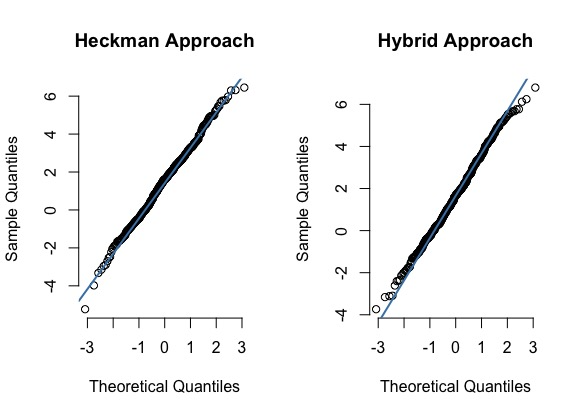
\includegraphics[scale=.35]{content/Figures/QQ_Zij_Design6.png}}
      \caption{\footnotesize{QQ plot of $\hat{z}_{12} - z_{12}$ in Design 6}}
      \label{QQ_Zij_Design6}
    \end{figure}
    With no fixed effects, the distributions are overall well approximated by a normal distribution.
\end{frame}

\begin{frame}
  \frametitle{Simulations: First stage QQ plot for single indices}
  \begin{figure}[htbp]
      \centerline{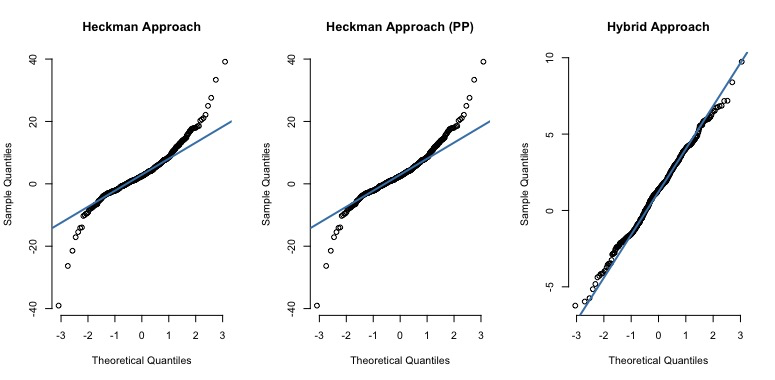
\includegraphics[scale=.35]{content/Figures/QQ_Zij_Design5.png}}
      \caption{\footnotesize{QQ plot of $\hat{z}_{12} - z_{12}$ in Design 5}}
      \label{QQ_Zij_Design5}
    \end{figure}
    In Design 5, the distributions for the Probit and Probit(PP) have heavier tails than the normal distribution $\xrightarrow{}$ mainly affected by the extreme value of fixed effects.
\end{frame}

\begin{frame}
  \frametitle{Simulations: First stage QQ plot for single indices}
  \begin{figure}[htbp]
      \centerline{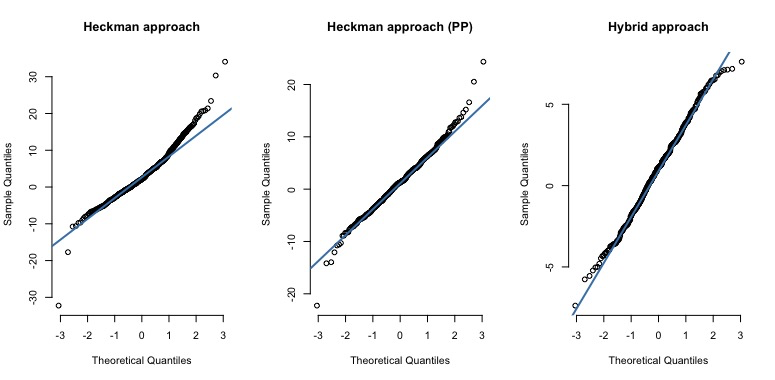
\includegraphics[scale=.35]{content/Figures/QQ_Zij_Design7.png}}
      \caption{\footnotesize{QQ plot of $\hat{z}_{12} - z_{12}$ in Design 7}}
      \label{QQ_Zij_Design7}
    \end{figure}
    In Design 7, the distributions for the Probit and Probit(PP) are more skewed $\xrightarrow{}$ mainly affected by the distribution of the structural parameters.
\end{frame}

\begin{frame}[label = qqplots]
    \frametitle{Simulation: observation equation}
    \begin{figure}[htbp]
        \centerline{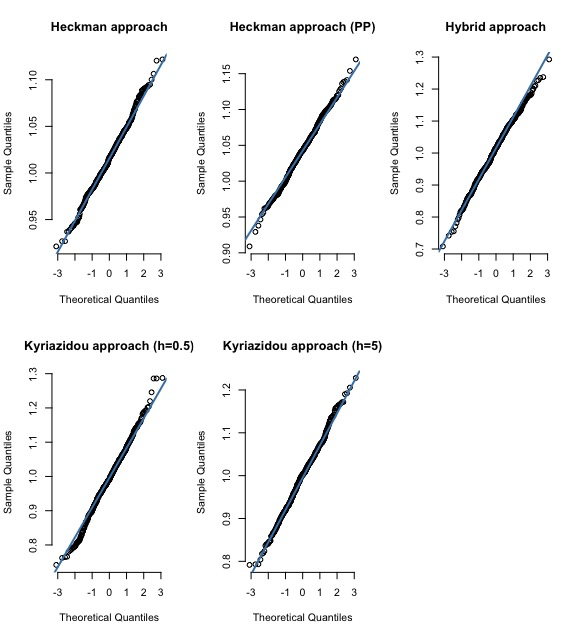
\includegraphics[scale=.3]{content/Figures/QQ_beta_11_Design5.png}}
        \caption{\footnotesize{QQ plot of estimated $\beta_{11}$ in Design 5}}
        \label{QQ_beta_11_Design5}
      \end{figure}
    \end{frame}
      \begin{frame}
        \frametitle{Simulation: observation equation}
      \begin{figure}[htbp]
        \centerline{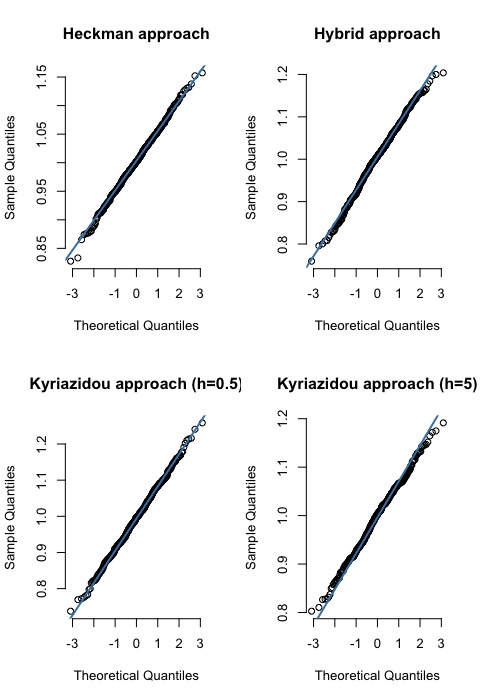
\includegraphics[scale=.3]{content/Figures/QQ_beta_11_Design6.png}}
        \caption{\footnotesize{QQ plot of estimated $\beta_{11}$ in Design 6}}
        \label{QQ_beta_11_Design6}
      \end{figure}
    \end{frame}
      \begin{frame}
        \frametitle{Simulation: observation equation}
      \begin{figure}[htbp]
        \centerline{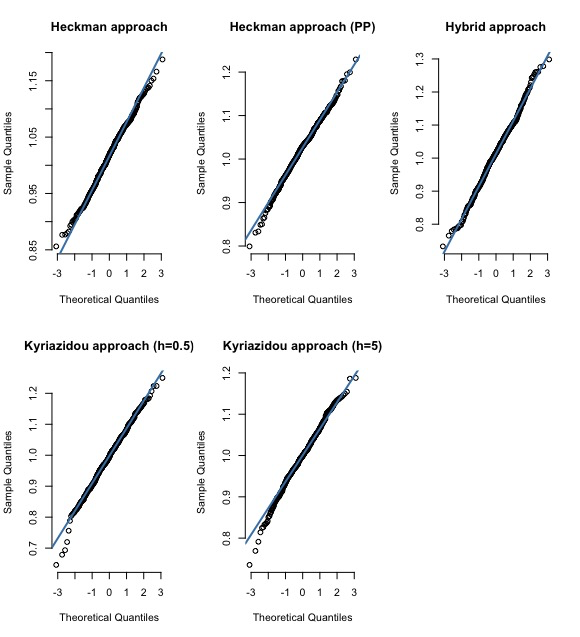
\includegraphics[scale=.3]{content/Figures/QQ_beta_11_Design7.png}}
        \caption{\footnotesize{QQ plot of estimated $\beta_{11}$ in Design 7}}
        \label{QQ_beta_11_Design7}
      \end{figure}
\end{frame}

\end{document}
